\title{Introdução à Web}
\date{\today}
\frame{\titlepage}

\begin{frame}{Agenda}
  \tableofcontents
\end{frame}

\section{História da Web}
\begin{frame}{Origem da Internet}
  \begin{itemize}
    \item \textbf{Década de 1960:} Projeto ARPANET - Defesa dos EUA cria a primeira rede de comunicação à prova de falhas.
    \item \textbf{Expansão:} A ARPANET se conecta a universidades, facilitando a pesquisa acadêmica e militar.
    \item \textbf{Protocolo TCP/IP:} Introduzido em 1983, fundamenta a comunicação na Internet moderna.
  \end{itemize}
\end{frame}

\begin{frame}{Criação da World Wide Web}
  \begin{itemize}
    \item \textbf{Tim Berners-Lee:} Físico no CERN, propôs um sistema de gerenciamento de informação em 1989.
    \item \textbf{Objetivo:} Facilitar o compartilhamento e atualização de informações entre pesquisadores.
    \item \textbf{Primeiro website:} Lançado em 1991, acessível externamente em 1993.
  \end{itemize}
\end{frame}

\begin{frame}{Evolução da Web: A Primeira Fase}
  \begin{itemize}
    \item \textbf{Web 1.0 (Década de 1990):} Era das páginas estáticas. Conteúdo criado por poucos, consumido por muitos.
    \item \textbf{Formatos de mídia:} Textos e imagens predominam, com pouca interatividade.
    \item \textbf{Ferramentas de busca:} Advento de motores de busca como Yahoo! e Google, facilitando a navegação.
  \end{itemize}
\end{frame}

\begin{frame}{Transição para a Web Dinâmica}
  \begin{itemize}
    \item \textbf{Web 2.0 (Início dos anos 2000):} Foco na interatividade, redes sociais e conteúdo gerado pelo usuário.
    \item \textbf{Aplicações web:} Surgimento de plataformas como Facebook, YouTube e Wikipedia.
    \item \textbf{Tecnologias chave:} JavaScript, AJAX e frameworks frontend revolucionam a criação de páginas dinâmicas.
  \end{itemize}
\end{frame}

\begin{frame}{A Web Moderna e o Futuro}
  \begin{itemize}
    \item \textbf{Web 3.0 e além:} Enfatiza a semântica, inteligência artificial, e a descentralização da internet.
    \item \textbf{Internet das Coisas (IoT):} A Web se expandindo além dos computadores, conectando dispositivos do dia a dia.
    \item \textbf{Desafios e oportunidades:} Privacidade, segurança da informação e a promessa de uma Web mais integrada e personalizada.
  \end{itemize}
\end{frame}


\section{Conceitos de Internet e Web}
\section{Conceitos de Internet e Web}
\begin{frame}{Internet vs. Web}
  \begin{itemize}
    \item \textbf{Internet:} Uma vasta rede de redes. Um sistema global de redes de computadores interconectadas que utilizam o protocolo de internet (TCP/IP) para se comunicarem.
    \item \textbf{Web (World Wide Web):} Um dos serviços disponíveis na Internet, permitindo a visualização de páginas interligadas por meio de navegadores.
    \item \textbf{Diferença Chave:} A Internet é a infraestrutura, enquanto a Web é um serviço construído sobre essa infraestrutura.
  \end{itemize}
\end{frame}

\begin{frame}{Como a Web Funciona - Parte 1}
  \begin{itemize}
    \item \textbf{URLs (Uniform Resource Locators):} Endereços usados para acessar páginas na Web.
    \item \textbf{Navegadores (Browsers):} Programas que interpretam e exibem as páginas da Web aos usuários.
    \item \textbf{Servidores Web:} Computadores que armazenam as páginas da Web e as disponibilizam aos usuários.
  \end{itemize}
\end{frame}

\begin{frame}{Como a Web Funciona - Parte 2}
  \begin{itemize}
    \item \textbf{Arquitetura Cliente-Servidor:} Modelo de comunicação onde os clientes solicitam recursos e os servidores respondem a essas solicitações.
    \item \textbf{Requisição e Resposta:} Processo básico de interação na Web, usando protocolos como HTTP.
    \item \textbf{Estado da Conexão:} HTTP é um protocolo sem estado, mas tecnologias como cookies e sessões permitem o rastreamento de sessões de usuário.
  \end{itemize}
\end{frame}

\begin{frame}{Protocolos da Web: HTTP}
  \begin{itemize}
    \item \textbf{HTTP (HyperText Transfer Protocol):} Fundamento da comunicação de dados na Web, definindo como as mensagens são formatadas e transmitidas.
    \item \textbf{Métodos HTTP:} GET para solicitar dados, POST para enviar dados, entre outros.
    \item \textbf{Códigos de Status:} Respostas do servidor, como 200 (OK), 404 (Not Found) e 500 (Internal Server Error).
  \end{itemize}
\end{frame}

\begin{frame}{Protocolos da Web: HTTPS}
  \begin{itemize}
    \item \textbf{HTTPS (HyperText Transfer Protocol Secure):} Versão do HTTP com camada adicional de segurança (SSL/TLS), protegendo a integridade e a confidencialidade dos dados durante a transferência.
    \item \textbf{Importância:} Fundamental para transações seguras, como compras online e operações bancárias.
    \item \textbf{Certificados Digitais:} Usados para autenticar a identidade do servidor, garantindo aos usuários que estão se conectando ao site correto.
  \end{itemize}
\end{frame}


\section{Arquitetura Cliente-Servidor}
\begin{frame}{Conceito de Cliente-Servidor}
  \begin{itemize}
    \item \textbf{Definição:} Modelo de arquitetura de rede que separa clientes e servidores, cada um com funções específicas.
    \item \textbf{Cliente:} Dispositivo ou programa que solicita serviços ou recursos.
    \item \textbf{Servidor:} Dispositivo ou programa que fornece serviços ou recursos aos clientes.
    \item \textbf{Interações:} Comunicação baseada em requisições (clientes) e respostas (servidores).
  \end{itemize}
\end{frame}

\begin{frame}{Aplicações Web na Arquitetura Cliente-Servidor}
  \begin{itemize}
    \item \textbf{Websites e Aplicações Web:} Exemplos primários de implementações cliente-servidor.
    \item \textbf{Comunicação:} Utiliza protocolos como HTTP/HTTPS para troca de informações.
    \item \textbf{Dinamismo:} Servidores processam solicitações e retornam conteúdo dinâmico baseado nas interações do usuário.
  \end{itemize}
\end{frame}

\begin{frame}{Benefícios da Arquitetura Cliente-Servidor}
  \begin{itemize}
    \item \textbf{Centralização de Recursos:} Facilita a gestão de dados e aplicações em um local centralizado.
    \item \textbf{Escalabilidade:} Adiciona mais servidores ou aumenta a capacidade para suportar mais clientes.
    \item \textbf{Manutenção e Atualizações:} Realizadas no servidor, afetam imediatamente todos os clientes conectados.
  \end{itemize}
\end{frame}

\begin{frame}{Desafios da Arquitetura Cliente-Servidor}
  \begin{itemize}
    \item \textbf{Segurança:} Necessidade de proteger tanto os servidores quanto as comunicações cliente-servidor.
    \item \textbf{Carga do Servidor:} Altas demandas podem sobrecarregar servidores, necessitando de técnicas de balanceamento de carga.
    \item \textbf{Dependência da Conexão:} A experiência do usuário pode ser afetada pela qualidade da conexão à Internet.
  \end{itemize}
\end{frame}

\begin{frame}{Evolução e Tendências Futuras}
  \begin{itemize}
    \item \textbf{Computação em Nuvem:} Aumenta a flexibilidade e reduz custos com infraestrutura física.
    \item \textbf{Microserviços:} Desenvolvimento e implementação de aplicações como uma coleção de serviços pequenos e independentes.
    \item \textbf{Descentralização:} Exploração de tecnologias como blockchain para criar arquiteturas menos centralizadas e mais seguras.
  \end{itemize}
\end{frame}

\section{Arquiteturas Modernas de Aplicações Web}

\begin{frame}{Visão Geral das Arquiteturas Modernas}
  \begin{itemize}
    \item As arquiteturas modernas estão evoluindo para \textbf{sistemas distribuídos}, focando em \textit{escalabilidade}, \textit{flexibilidade} e \textit{independência de serviço}.
    \item Componentes chave incluem \textbf{serviços}, \textbf{APIs}, \textbf{API Gateways}, e \textbf{bancos de dados isolados}.
    \item Esses sistemas são projetados para \textit{facilitar a manutenção}, \textit{atualizações rápidas} e \textit{a entrega contínua de software}.
  \end{itemize}
\end{frame}

\begin{frame}[fragile]
  \frametitle{Frameworks mais usados em 2023}
  \begin{figure}
    \centering
    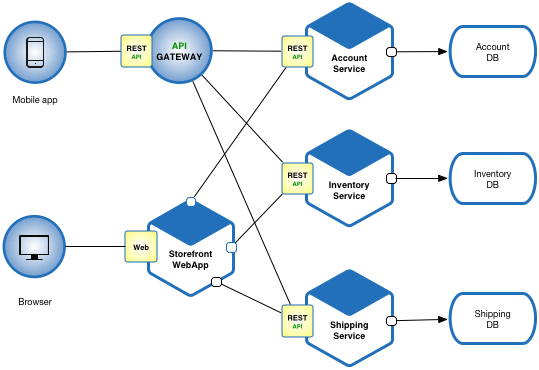
\includegraphics[width=0.8\textwidth]{assets/architecture.png}
    \caption{Frameworks mais usados}
  \end{figure}
\end{frame}

\begin{frame}{Serviços em Arquiteturas Modernas}
  \begin{itemize}
    \item \textbf{Microserviços:} Aplicações são divididas em pequenos serviços independentes, cada um responsável por uma função específica.
    \item Cada serviço é \textit{autônomo} e pode ser desenvolvido, implantado e escalado \textit{independentemente}.
    \item Favorece a \textbf{diversidade tecnológica}, permitindo que diferentes serviços usem diferentes stacks tecnológicas.
  \end{itemize}
\end{frame}

\begin{frame}{APIs: Ponte para a Comunicação}
  \begin{itemize}
    \item \textbf{APIs (Application Programming Interfaces)} servem como pontes para a comunicação entre serviços, aplicativos e sistemas.
    \item Facilitam a \textit{integração e a interoperabilidade} entre diferentes componentes de software e serviços de terceiros.
    \item Utilizam padrões como \textbf{REST} e \textbf{GraphQL} para otimizar a comunicação e o tráfego de dados.
  \end{itemize}
\end{frame}

\begin{frame}{API Gateways}
  \begin{itemize}
    \item O \textbf{API Gateway} atua como um intermediário que \textit{gerencia solicitações de entrada}, direcionando-as para os serviços internos apropriados.
    \item Oferece \textit{autenticação}, \textit{rate limiting}, e \textit{caching} para melhorar a segurança e a eficiência.
    \item Simplifica a arquitetura do cliente, oferecendo um ponto único de entrada para várias APIs e serviços.
  \end{itemize}
\end{frame}

\begin{frame}{Bancos de Dados Isolados}
  \begin{itemize}
    \item Em arquiteturas baseadas em microserviços, cada serviço geralmente possui seu \textbf{próprio banco de dados isolado}, garantindo \textit{segurança} e \textit{independência de dados}.
    \item Isso permite que os serviços sejam \textit{escalados ou modificados} sem afetar outros serviços.
    \item Apoia a \textbf{consistência} e a \textbf{integridade dos dados} em ambientes distribuídos e altamente disponíveis.
  \end{itemize}
\end{frame}

